\chapter{Barreiras para contribuir com software livre}
\label{barreirasSL}

O software livre se apresenta atualmente como um modelo já consolidado e viável
em um número crescente de aplicações e ambientes. No entanto, restam incertezas
jurídicas e dificuldades, por exemplo com patentes de software, possíveis problemas de
interoperabilidade com plataformas e protocolos criados e baseados em implementações
não-livres e a necessidade de demonstrar a viabilidade econômica do modelo em mais
casos e contextos. Alguns desses desafios estão vinculados às barreiras criadas pelo
modelo e cultura do software restrito~\cite{kon2012software}.

Além dessas dificuldades técnicas enfrentadas por projetos de software livre, existe 
também a dificuldade de se encontrar e estabelecer novos contribuidores para seus os
projetos. Dessa forma o objetivo da pesquisa de~\citeonline{steinmancher2015} foi encontrar as barreiras enfrentadas 
por novos contribuidores para começar a contribuir com projetos de software livre, 
não importando saber o motivo que levava os novos contribuidores
a escolher um projeto de software livre, mas as tarefas que ele tinha que fazer após
ter escolhido um projeto.

O processo de entrada de um novo contribuidor a um projeto de software livre é complexo
e composto de diferentes estágios, pode-se considerar 4 diferentes forças que influenciam 
esse processo: motivação do novo contribuidor, atratividade do projeto, barreiras de entrada
no projeto e retenção do projeto\\~\cite{Steinmacher:2014:HLO:2593702.2593704, 2049}.

Para entender as barreiras encontradas por novos contribuidores durante a entradas dos
mesmo nos projetos foi feita uma análise qualitativa feita com diferentes estudantes em
diferentes projetos de software livre que foram consultados através de questionários
e entrevistas~\cite{Steinmacher:2014:HLO:2593702.2593704}.

Os dados dos questionários foram analisados conforme a \textit{Grounded Theory},
que se baseia no conceito da codificação, que é o processo de atribuição de um código
para efeitos de classificação ou identificação, e pode ser dividido em 3 passos:

\begin{itemize}

\item Codificação aberta, onde os conceitos são indentificados e suas propriedades e dimensões
são descobertos através dos dados.

\item Codificação \textit{axial}, onde são feitas as conexões dos dados identidicados e 
agrupados de acordo com suas propriedades para representar categorias.

\item Seleção de código, onde cada categoria é identificada e descrita~\cite{strauss1998basics}.

\end{itemize}

Na primeira análise dos resultados de acordo com a \textit{Grounded Theory} surgiram 
38 barreiras que foram divididas em 7 categorias com suas respectivas barreiras:

\begin{itemize}

\item Tarefas para levantar o ambiente: 

	\begin{itemize}
	\item Tarefas para levantar o ambiente; 
	\item Dependências das plataformas;
	\item Problemas para achar o repositório oficial;
	\item Problemas com bibliotecas.
	\end{itemize}

\item Tarefas de código:
	
	\begin{itemize}
	\item Tamanho do código;
	\item Má qualidade do código;
	\item Falta de padrões de código;
	\item Problemas para entender o código;
	\item Código desatualizado.
	\end{itemize}

\item Problemas com a documentação:

	\begin{itemize}
	\item Falta de documentação;
	\item Falta de documentação da estrutura do projeto;
	\item Falta de documentação para levantar o ambiente;
	\item Falta de documentação do processo de contribuição no projeto;
	\item Documentação desatualizada;
	\item Documentação confusa;
	\item Documentação espalhada;
	\item Falta de comentários no código;
	\item Falta de documentação de \textit{Design};
	\item Falta de documentação do código.
	\end{itemize}

\item Comportamento do novo contribuidor:

	\begin{itemize}
	\item Falta de compromisso do novo contribuidor;
	\item Subestimar o desafio de começar a contribuir;
	\end{itemize}

\item Conhecimentos técnicos do novo contribuidor:

	\begin{itemize}
	\item Falta de conhecimento nas ferramentas utilizadas pelo projeto;
	\item Conhecimento prévio em ferramentas de controle de versão;
	\item Dificuldade de escolher a ferramenta certa;
	\item Falta de conhecimento nas tecnologias utilizadas no projeto;
	\item Linguagem de programação utilizada;
	\item Curva de aprendizado;
	\item Curva de aprendizado das ferramentas do projeto;
	\item Falta de conhecimento geral.
	\end{itemize}

\item Encontrando uma maneira de começar:
	
	\begin{itemize}
	\item Encontrar uma tarefa para começar;
	\item Encontrar a parte certa do código para trabalhar;
	\item Lista de \textit{bugs} desatualizada.
	\end{itemize}

\item Tarefas de interação social:
	
	\begin{itemize}
	\item Econtrar alguém para ajudar;
	\item Demora na resposta dos e-mails;
	\item Respostas rudes as dúvidas;
	\item Uso de termos intimidadores;
	\item Tarefas de comunicação;
	\item Encontrar um mentor.
	\end{itemize}

\end{itemize} 

A análise qualitativa ajudou a encontrar barreiras e a relação entre as barreiras
que influenciam um novo contribuidor de um de software livre
\\~\cite{Steinmacher:2014:HLO:2593702.2593704}.

Após uma segunda análise dos resultados com os dados dos formulários de contribuidores 
que demoraram um pouco mais para responder aos questionários foram identificadas 
50 barreiras, divididas em 6 categorias~\cite{6943482}. 

As novas barreiras identificadas em suas categorias foram:

\begin{itemize}

\item Tarefas de recepção de novos contribuidores, a recepção dos novos contribuidores às 
comunidades ficou mais evidente como de extrema importância pois quando o novo 
contribuidor não se sente confortável na comunidade ele rapidamente fica desmotivado.
	\begin{itemize}
	\item Respostas de dúvidas a novos contribuidores de forma ``não amigável'';
	\item Demora para receber as respostas;
	\item O não recebimento de respostas pelos novos contribuidores;
	\item Respostas não educadas.
	\end{itemize}

\item Características dos novos contribuidores, esta categoria engloba duas características
citadas anteriormente, Comportamento do novo contribuidor e Conhecimentos técnicos do novo
contribuidor e foram encontradas barreiras na segunda análise que ainda não estavam nessas
categorias, são elas:

	\begin{itemize}
	\item Falta de proatividade dos novos contribuidores;
	\item Necessidade de ser paciente;
	\item Falta de comprometimento dos novos contribuidores;
	\item O não reconhecimeto das respostas;
	\item Timidez dos novos contribuidores;
	\item Nível de inglês dos novos contribuidores;
	\item Fazer comentários úteis nas listas de e-mail e fóruns;
	\item Não enviar mensagens corretas e significativas nas listas;
	\item Falta de conhecimento adequado em liguagens de programação;
	\item Falta de conhecimento na tecnologia e nas ferramentas utilizadas no projeto;
	\item Falta de conhecimento prévio em versionamento e ferramentas de controle de 
versão;
	\item Falta de conhecimento em teste unitário.
	\item Dificuldade em encontrar ferramentas adequadas para o desenvolvimento.
	\end{itemize}
 
\item Novos contribuidores necessitam de orientação, os novos contribuidores precisam
que lhes diguem a maneira como eles devem contribuir com o projeto e onde. Novas barreiras
relacionadas a esta categoria foram encontradas:
	
	\begin{itemize}
	\item Realizar tarefas;
	\item Incompleto manual de como contribuir;
	\item Novos contribuidores não sabem o que é um modelo de contribuição.
	\end{itemize}

\item Problemas com a documentação, já haviam sido identificadas as barreiras para esta categoria.

\item Barreiras técnicas, esta categoria foi dividida em outras 3 subcategorias que englobam
a categoria citada anteriormente como Tarefas de código e a categoria Tarefas para levantar o ambiente.
	
	\begin{itemize}
	\item Barreiras de código e arquitetura;
		\begin{itemize}
		\item Má qualidade do \textit{Design};
		\item Má qualidade do código;
		\item Complexidade do código;
		\item Tamanho do código;
		\item Entendimento da arquitetura e da estrutura do código;
		\item Entendimento do código;
		\item Entendimento do fluxo da informação no projeto;
		\end{itemize}
	\item Barreiras para submeter as contribuições;
		\begin{itemize}
		\item Demora na revisão das contribuições;
		\item Ter uma contribuição aceita;
		\item Falta de informação de como enviar uma contribuição;
		\item Tarefa de criar um \textit{pacth}.
		\end{itemize}
	\item Barreiras para levantar o ambiente.
		\begin{itemize}
		\item Criando um espaço de trabalho local;
		\item Dependências de bibliotecas;
		\item Dependências de plataforma;
		\item Encontrar o correto código fonte.
		\end{itemize}
	\end{itemize}

\item Diferenças culturais, esta categoria é resultado de problemas de interação, 
alguns projetos de software livre tem escala global de desenvolvimento e isso
gera esses problemas.
	\begin{itemize}
	\item Alguns contribuidores prescisam de contato com pessoas;
	\item Mensagem recebida é considerada rude.
	\end{itemize}
	
\end{itemize}

Após a obtenção do modelo com a análise dos questionários foi feita uma reanálise
de todos os dados obtidos para a criação de um modelo único que acomodasse todas
as barreiras encontradas, dessa forma algumas barreiras foram agrupadas em uma única e 
as categorias foram reorganizadas~\cite{6943482}.

O novo modelo tem 58 barreiras agrupadas em 6 categorias conforme a Figura \ref{livre}
\\\cite{Steinmacher:2016:OOS:2884781.2884806}.

\begin{figure}[h]
	\centering
		\includegraphics[keepaspectratio=true,scale=0.28]{figuras/Barreiras.eps}
	\caption{Barreiras para contribuir com Software livre.}
	\label{livre}
\end{figure}

\section{O portal para suporte a novos contribuidores: FLOSSCoach}
\label{flosscoach}

A fim de mitigar as barreiras encontradas, ~\citeonline{steinmancher2015} criou um portal~\footnote{http://flosscoach.com/} 
onde para cada software são apresentadas todas as informações para que cada barreira seja sanada.

\begin{figure}[h]
	\centering
	\label{portalFlossCoach}
		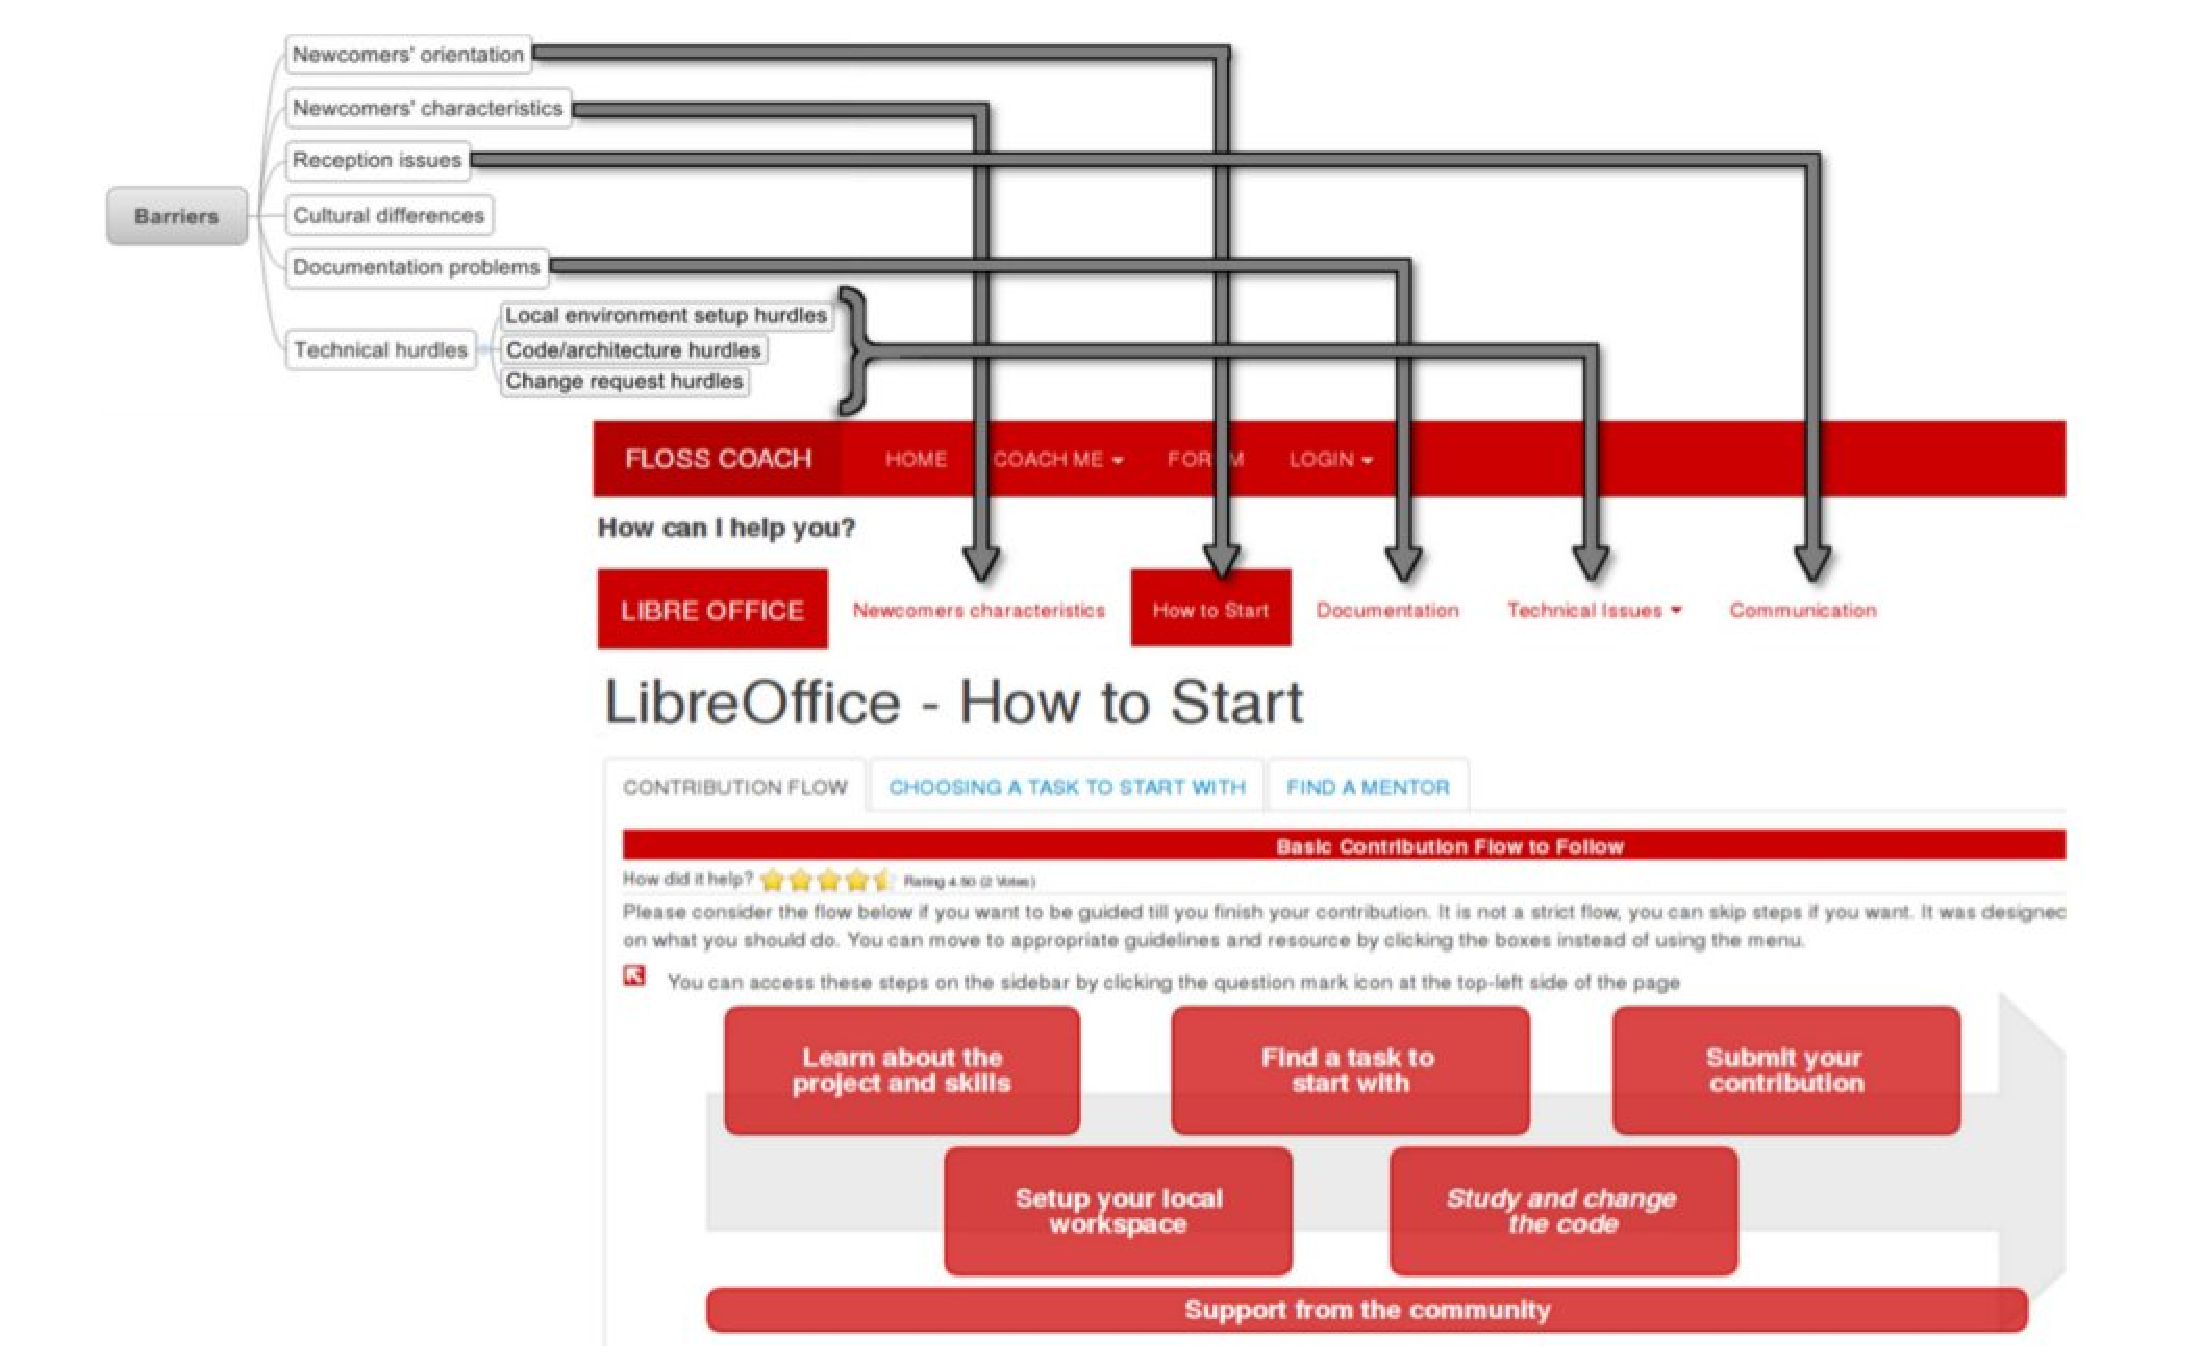
\includegraphics[keepaspectratio=true,scale=0.4]{figuras/portal.eps}
	\caption{Portal para suporte a novos contribuidores.}
\end{figure}

Cada categoria apresentada passou a ser uma aba do portal e dentro de cada aba 
estão as informações de cada barreira. Eles desenvolveram o portal em inglês
para que atenda um número maior de contribuidores.

A aba \textit{How to Start} estão contidas as orientações aos novos contribuidores, os novos
contribuidores tem dificuldade de se familiarizar com a comunidade e com os processos
para contribuir e necessitam de orientação adequada para começar corretamente a
contribuir com o projeto.

Em \textit{Newcomers’ characteristics}(Características dos novos contribuidores) são 
compreendidas as barreiras relacionadas à experiência e o comportamento dos novos 
contribuidores e a maneira com que devem começar a interagir com a comunidade.

Em \textit{Communication}, é relatado como são as interações entre 
os membros da comunidade e compreende as barreiras de Tarefas de recepção.

Na aba \textit{Documentation} tem os documentos que o novo contribuidor precisa ler 
para se inteirar dos aspectos técnicos e sociais da comunidade.

Por fim, na aba \textit{Technical issues}, estão as dificuldades técnicas que os novos
contribuidores irão enfrentar ao ter o primeiro contato com o código e para levantar
o ambiente~\cite{steinmancher2015}.

Esta primeira versão do FlossCoach é estático e apenas quem pode cadastrar novos projetos 
são os criadores diretamente no código da aplicação, desta forma o usuário ao fazer login
na aplicação, pode apenas fazer comentários ao conteúdo disponível de cada projeto.

Foi desenvolvido em \textit{Joomla}\footnote{https://www.joomla.org/}, que 
é um sistema de gestão de conteúdo. O núcleo deste sistema fornece funcionalidades que
são usadas de base para aplicações \textit{web} e sua vantagem é de ser facilmente 
utilizada por \textit{designers} inexperientes\\~\cite{Priefer:2016:JMD:2889160.2889176}.

O principal objetivo desse trabalho não é contribuir com o desenvolvimento do portal FlossCoach,
mas a engenharia de software se trata de construir e melhorar os produtos de software,
por esse motivo iniciamos o processo de construção do novo portal FlossCoach com
a intenção de aprimorar o portal para que ele possua as funcionalidades esperadas e 
seja mais utilizado por desenvolvedores de software.







